% !TeX encoding = UTF-8
% !TeX spellcheck = en_US
\documentclass[11pt]{article}
\usepackage[utf8]{inputenc}
\usepackage{indentfirst}
\usepackage[a4paper]{geometry}
\usepackage{graphicx}
\usepackage{float}
\usepackage[hidelinks]{hyperref}
\usepackage[bottom]{footmisc}
\usepackage{caption}

\title{Documentation}
\author{Jorge López Fueyo \\ 71779245V \\ UO245115}

\setlength{\parskip}{3mm plus 1mm minus 1mm}

\geometry{top = 20mm, bottom = 20mm, left = 30mm, right = 30mm}


\begin{document}	
	\newenvironment{qn}{\par\noindent\begin{minipage}{\linewidth}}{\end{minipage}\par}
	
	
	\pagenumbering{gobble}
	\maketitle
	\newpage
	\pagenumbering{arabic}

	\section{Introduction}
   
	In this work, we have been developing a desktop application that will allow the user to book and pay for a Cruise.

	The application is supposed to read the information from a set of files and, at the end of the process, store the result in a text file, including all the necessary booking information, such as the user contact data and the cruise data. At the end of the process, the user must be able to export the bill as a text file into a local directory.
   
	A system that keeps track of the orders has been implemented, so it is not allowed to book more than the available rooms of a ship.
   
	\section{Prototype}
	Our team's prototype\footnote{\url{https://moqups.com/jorgelopezfueyo@gmail.com/nN2oP7pI}} did not change much between the initial design and the final one, just an issue related with cash payment.
   
	The prototype consisted on 5 screens:
	\begin{qn}
		\begin{itemize}
			\item Initial panel: showing sponsored offers and a search bar.
		\end{itemize}
		\begin{center}
			\begin{minipage}{0.5\linewidth}
				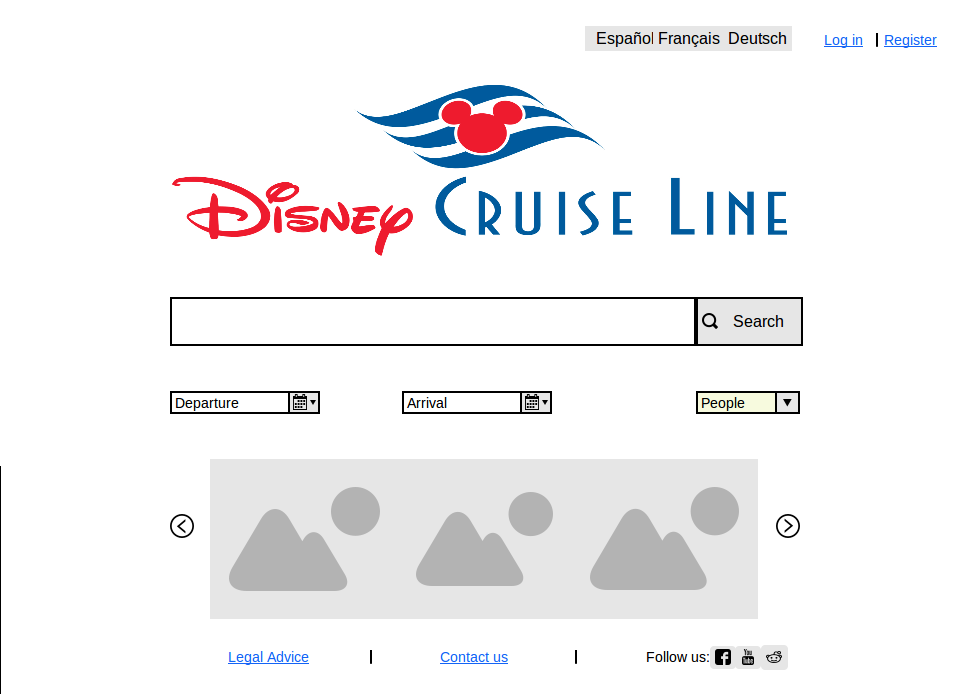
\includegraphics[width=\linewidth]{images/mockup1.png}
				\label{fig:mockup1}
			\end{minipage}
		\end{center}
	\end{qn}
	\begin{qn}
		\begin{itemize}
			\item Search panel: shows the results of the search. It also hast a search bar at the top.
		\end{itemize}
		\begin{center}
			\begin{minipage}{0.5\linewidth}
				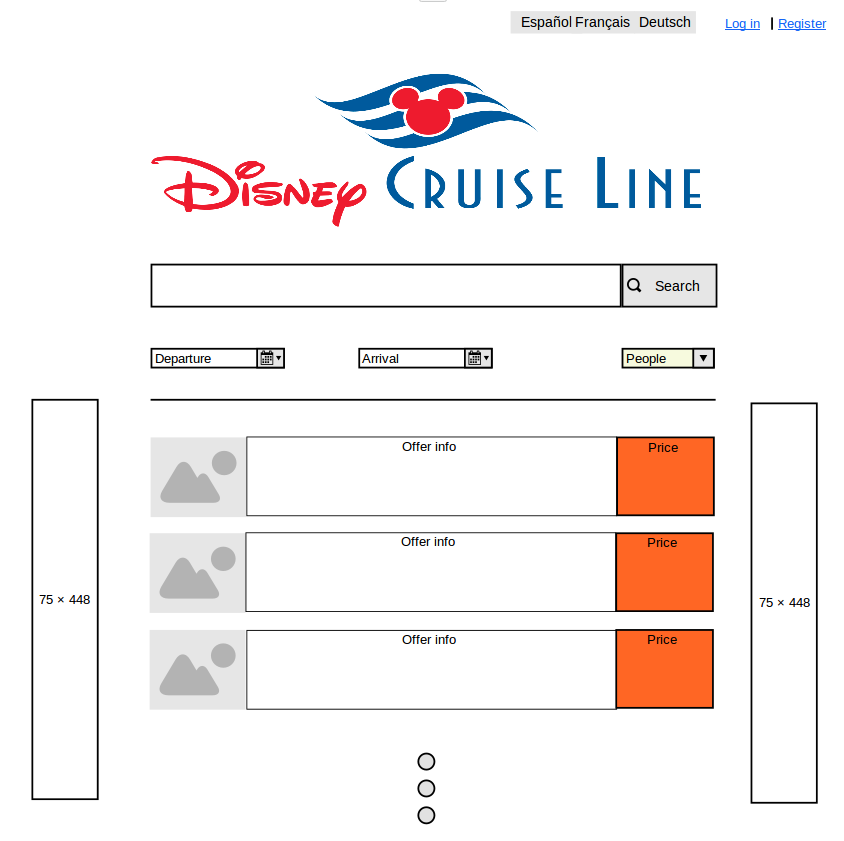
\includegraphics[width=\linewidth]{images/mockup2.png}
				\label{fig:mockup2}
			\end{minipage}
		\end{center}
	\end{qn}
	\begin{qn}
		\begin{itemize}
			\item Cruise panel: shows the information of the selected cruise, e.g. description or pictures. There is a a panel on the right allowing to book it.
		\end{itemize}
		\begin{center}
			\begin{minipage}{0.5\linewidth}
				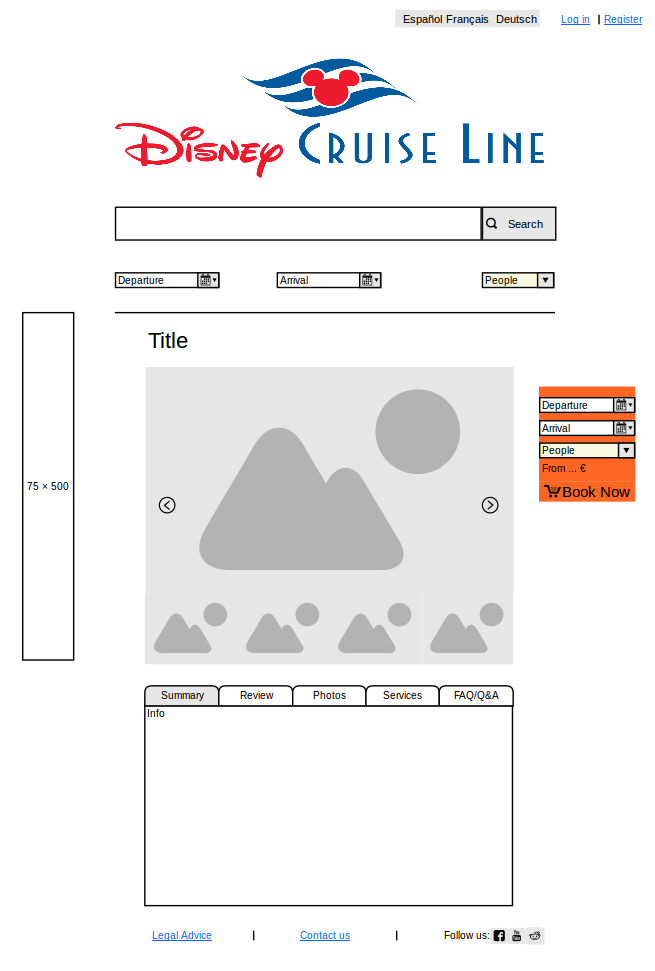
\includegraphics[width=\linewidth]{images/mockup3.png}
				\label{fig:mockup3}
			\end{minipage}
		\end{center}
	\end{qn}
	\begin{qn}
		\begin{itemize}
			\item Info panel: ask for the needed information such as people per cabin, extras or personal details. Allows to add the cruise to the cart and continue buying or just go ahead and pay.
		\end{itemize}
			\begin{center}
			\begin{minipage}{0.5\linewidth}
				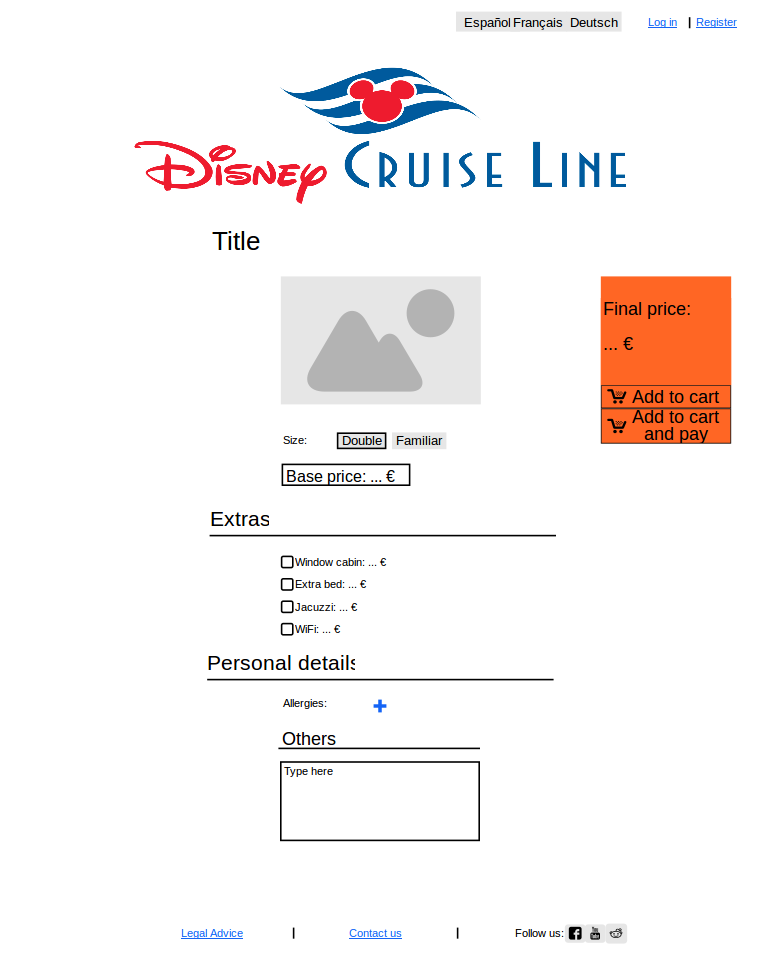
\includegraphics[width=\linewidth]{images/mockup4.png}
				\label{fig:mockup4}
			\end{minipage}
		\end{center}
	\end{qn}
	\begin{qn}
		\begin{itemize}
			\item Payment panel: allows the user to choose between various payment methods in order to pay the order. 
		\end{itemize}
		\begin{center}
			\begin{minipage}{0.5\linewidth}
				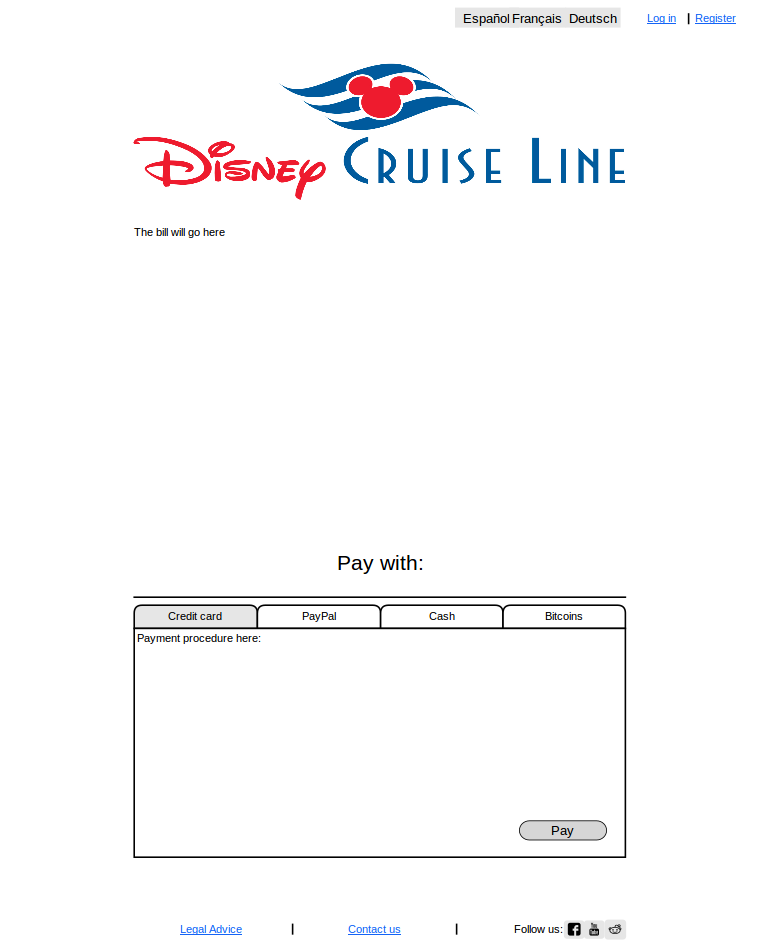
\includegraphics[width=\linewidth]{images/mockup5.png}
				\label{fig:mockup5}
			\end{minipage}
		\end{center}
	\end{qn}
   
	\section{Application}
	The application was coded using Java 8 version and IntelliJ IDEA as IDE. Builds where made using Gradle\footnote{\url{http://gradle.org/}} and the most of the libraries were imported using the mechanisms it provides. During the development, it has been hosted in a GitHub repository\footnote{\url{http://github.com/nokutu/trabajo-cpm}}. The application is using the following libraries:
	\begin{itemize}
	   	\item \textbf{Jasypt}\footnote{\url{www.jasypt.org/}}: security library used for password hashing.
	   	\item \textbf{Miglayout}\footnote{\url{http://miglayout.com/}}: powerful layout used in most JPanels.
	   	\item \textbf{JavaHelp}: needed for user help support.
	   	\item \textbf{Commons-Validator}: used to check if the emails addresses are valid.
	\end{itemize}
	\subsection{Design}
	The application was designed without the use of Window Builder, as, in my opinion, even though it makes things more visual, the code it creates is quite "spaghetti" and not very well structured.
   
	I have been using mainly 2 different layouts. \textbf{BorderLayout} in all the tabs of the \textbf{CardLayout} and in the JDialogs and \textbf{MigLayout}, which is an improved  version of \textbf{GridBagLayout} that allows to input constraints as a String containing commands.
   
   	\begin{qn}
	The application design consists of a \textbf{MainFrame} instance, whose content pane has a \textbf{CardLayout}. It contains:
		\begin{itemize}
		    \item \textbf{InitialPanel}: The first panel you see when the application is opened. It just contains the application's  logo and a search bar. The logo always links to this initial panel. At the top of the panel there is a NavBar. This component allows the user to login or register and, if already logged in, allows to modify his information or logout. Figure \ref{fig:initial}.
		\end{itemize}
		\begin{center}
			\begin{minipage}{0.8\linewidth}
			   	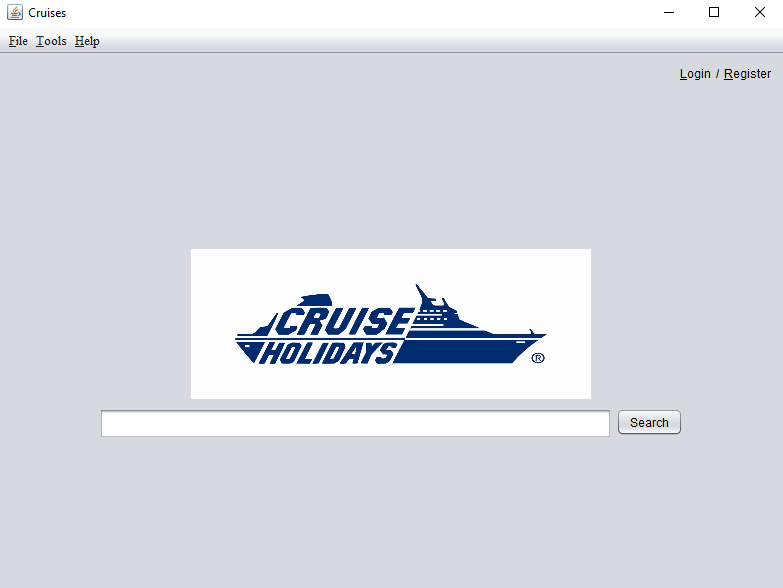
\includegraphics[width=\linewidth]{images/initial.png}
			   	\captionof{figure}{Initial panel}
			   	\label{fig:initial}
			\end{minipage}
		\end{center}
	\end{qn}
	
	\begin{qn}
		\begin{itemize}
	   	    \item \textbf{SearchPanel}: Displays the search results and allows the user to rerun searches. Each search result has its own JPanel and they are arranged in a vertical list. Figure \ref{fig:search}.
	   	\end{itemize}
	   	\begin{center}
			\begin{minipage}{0.8\linewidth}
				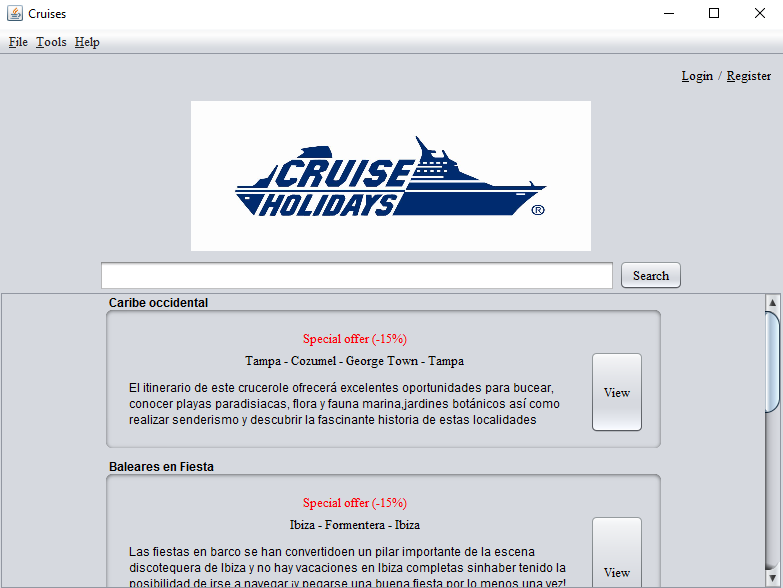
\includegraphics[width=\linewidth]{images/search.png}
				\captionof{figure}{Search panel}
				\label{fig:search}
			\end{minipage}
	    \end{center}
	\end{qn}
	
	\begin{qn}
	    \begin{itemize}
		    \item \textbf{CruisePanel}: Displays the information about the selected cruise, such as pictures, description and route. A \textbf{BookPanel} is shown on the right size, that allows to select the type of cabin, date, extras and people. Figure \ref{fig:cruise}.
		\end{itemize}
		\begin{center}
			\begin{minipage}{0.8\linewidth}
				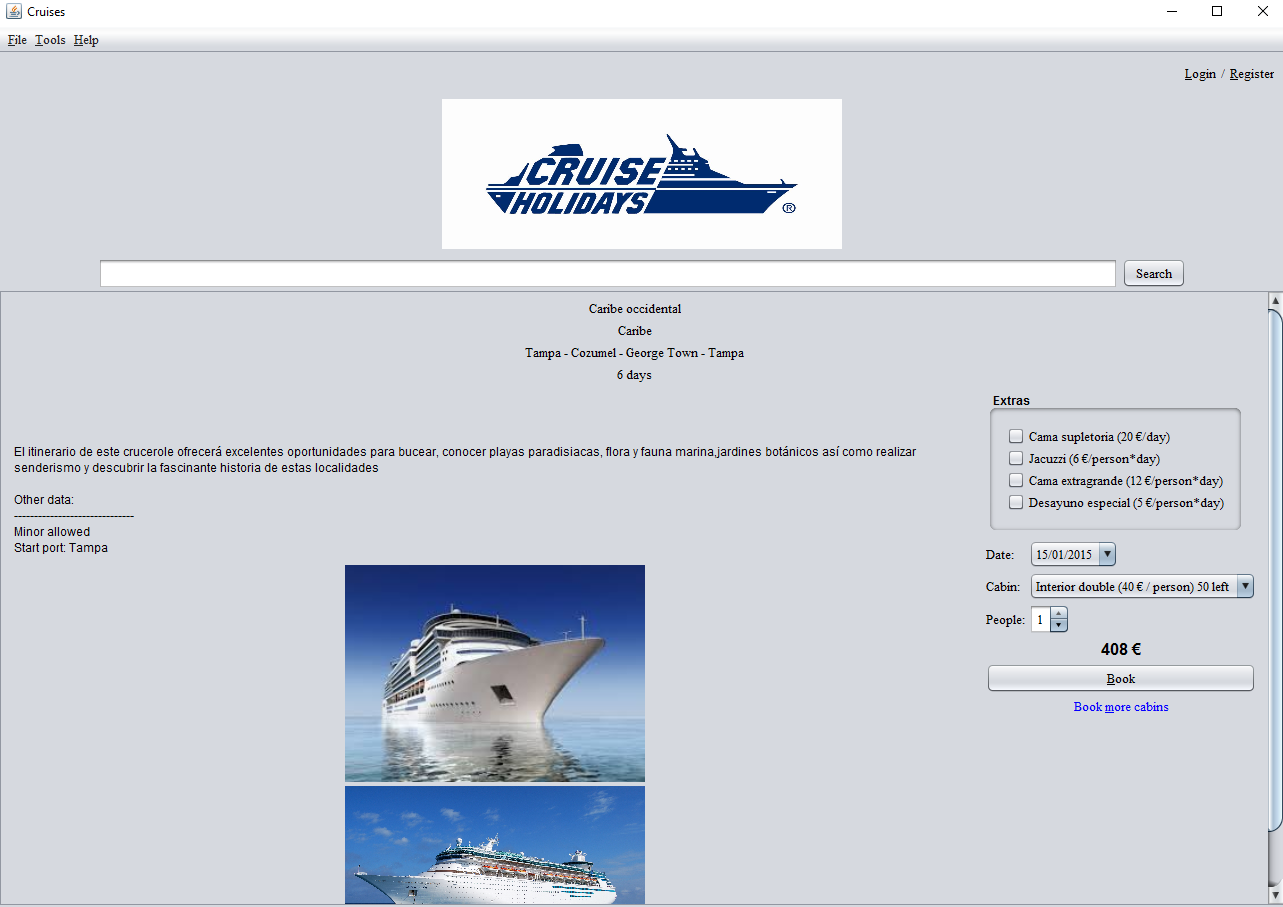
\includegraphics[width=\linewidth]{images/cruise.png}
				\captionof{figure}{Cruise panel}
				\label{fig:cruise}
			\end{minipage}
		\end{center}
	\end{qn}
	
	\begin{qn}
		\begin{itemize}
	   	    \item \textbf{PassengerInfoPanel}: In this panel the user is asked about the name and age of all the passengers in the cabin. It also checks for incompatibilities such as no minor in a room with a supplementary beds of minor in a non minor cruise. An individual JPanel with as many JTextFields as people in the cabin is create for each booked cabin, then they are arranged as a 2 column table. Figure \ref{fig:passenger}.
	    \end{itemize}
	    \begin{center}
		    \begin{minipage}{0.8\linewidth}
		   	   	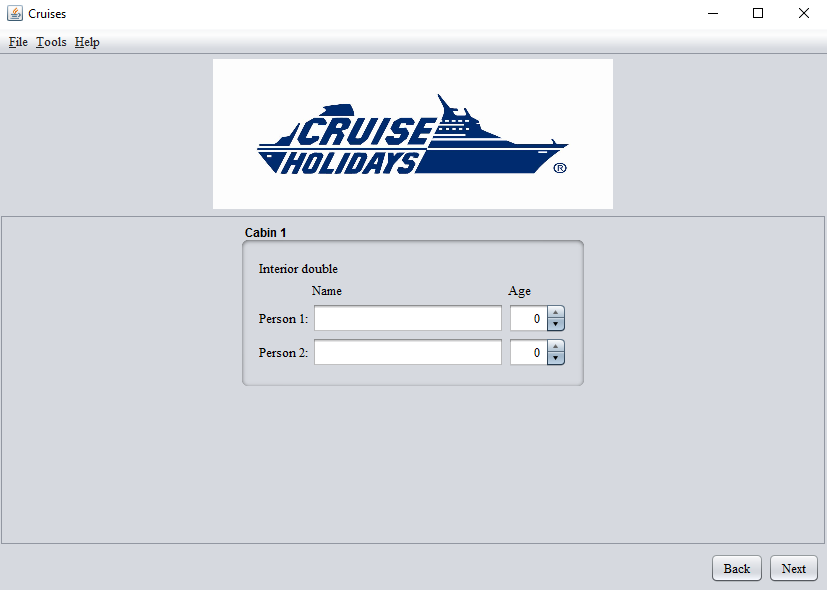
\includegraphics[width=\linewidth]{images/passenger.png}
		   	   	\captionof{figure}{Passenger information panel}
		   	   	\label{fig:passenger}
		    \end{minipage}
	    \end{center}
    \end{qn}
    
    \begin{qn}
    	\begin{itemize}
	   	    \item \textbf{PaymentPanel}: Displays the final price of the booking. A bill, which contains all the information required, is shown in the middle of the screen. From here the user can open a new dialog in order to enter the payment information. In the case the user isn't logged in yet, only a JLabel asking him to log in or register will be shown. Figure \ref{fig:payment}.
   	    \end{itemize}
   	    \begin{center}
	   	    \begin{minipage}{0.8\linewidth}
		   	   	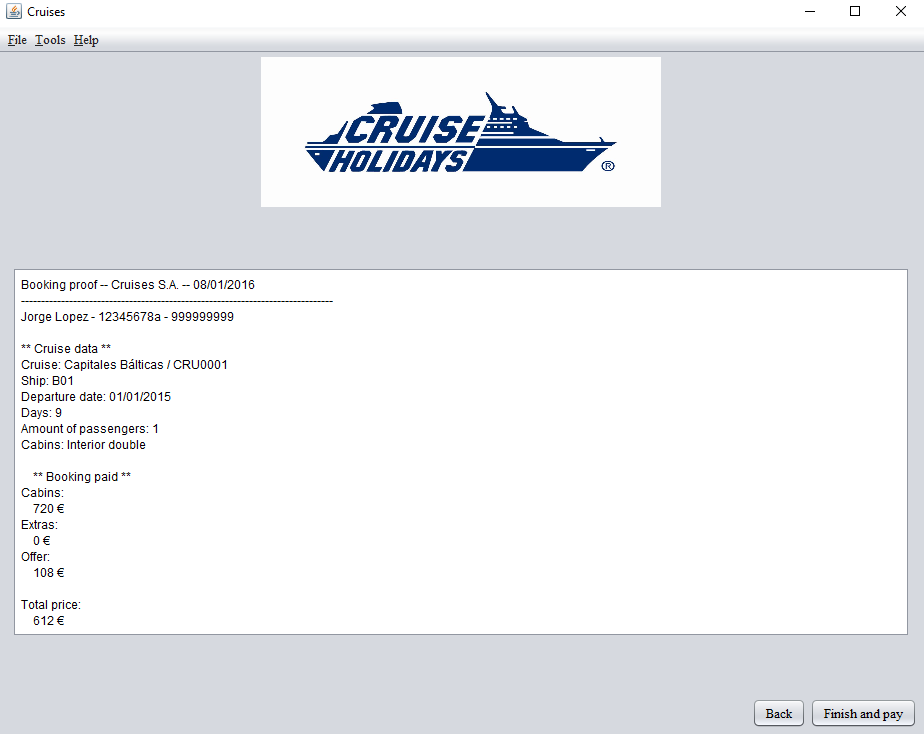
\includegraphics[width=\linewidth]{images/payment.png}
		   	   	\captionof{figure}{Payment panel}
		   	   	\label{fig:payment}
	   	    \end{minipage}
   	    \end{center}
   	\end{qn}
   	
   	\begin{qn}
		\begin{itemize}
			\item \textbf{FinalPanel}: Displays the bill again and allows the user to export it into a local directory. Figure \ref{fig:final}.
		\end{itemize}   
		\begin{center}
			\begin{minipage}{0.8\linewidth}
				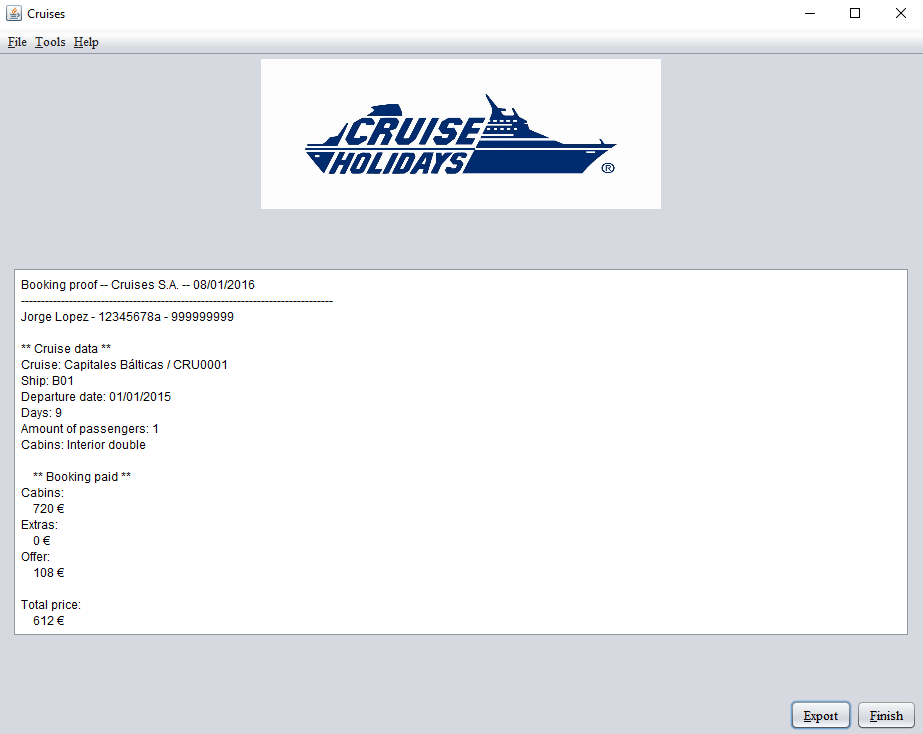
\includegraphics[width=\linewidth]{images/final.png}
				\captionof{figure}{Final panel}
				\label{fig:final}
			\end{minipage}
		\end{center}
	\end{qn}

   
	\subsection{Logic}
	At the start, the application has the input files. The ".dat" files should be located at the base folder and the images should be located inside a folder called images.
   
	The main logic classes are:
	\begin{itemize}
		\item \textbf{Database}: The main part of the application's logic is related with this class. It stores all ships, zones, cruises, cities and users of the application. In the case of users, the password is stored using a hashing algorithm from the library Jasypt.
		\item \textbf{Preferences}: When the application is running, the preferences, such as the list of users registered or the personal settings are stored inside a HashMap in this class. Whenever the application is closed, they are saved into a text file located into the user directory, inside a folder called ".cruises". This file is then loaded when the application is started again.
		\item \textbf{I18n}: Stores the used internationalization methods:
		\begin{itemize}
			\item \textbf{tr(String)}: just translates the given key.
			\item \textbf{trn(String, int)}: translates the given key depending on the integer. If it is different from one, it will return the plural and the singular otherwise.
			\item \textbf{trc(String, Object[])}: translates the given key substituting the given Object inside.
		\end{itemize}
   \end{itemize}

\end{document}